\documentclass{article}
\usepackage[a4paper,margin=1in]{geometry}
\usepackage{tikz}
\usetikzlibrary{arrows.meta,automata,positioning}

\title{CSE411 Assignment \#1: The NFA/DFA for \texttt{IF \(\mid\) ID \(\mid\) INT}}
\author{Sungho Kim (20241065)}
\date{\today}

\begin{document}
\maketitle

\section{NFA}
\begin{center}
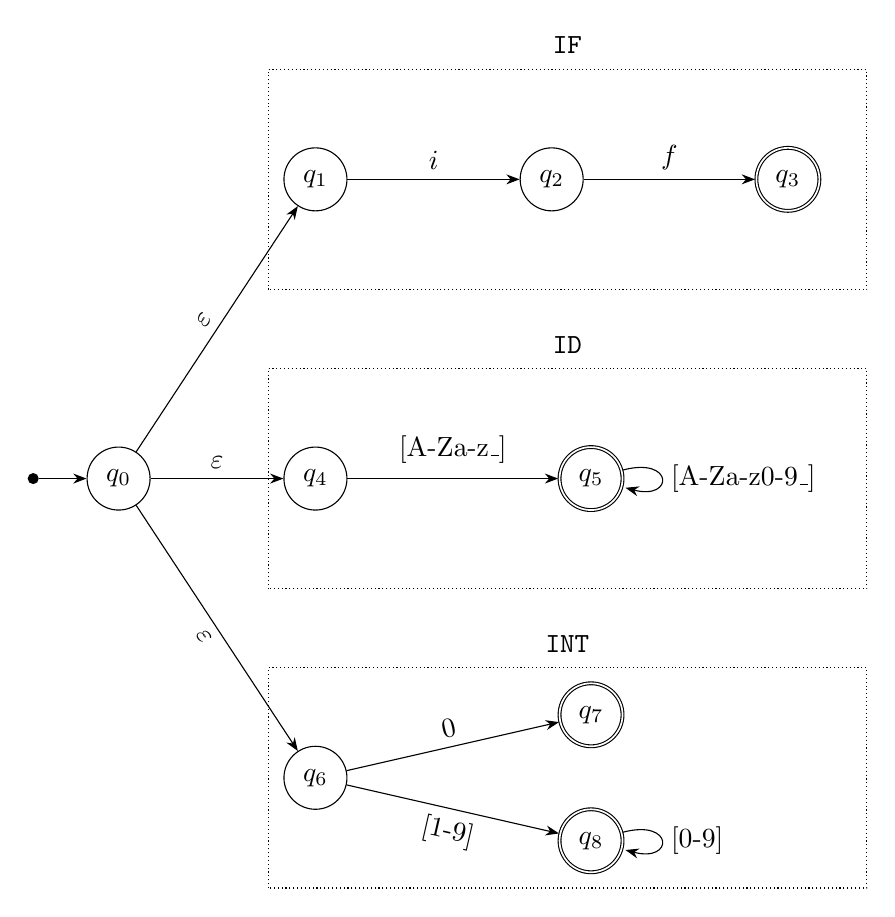
\begin{tikzpicture}[->, >=Stealth, every state/.style={minimum size=8mm}]
\node[state] (q0) at (0,0) {$q_0$};
\node[state] (q1) at (2.5,3.8) {$q_1$};
\node[state] (q2) at (5.5,3.8) {$q_2$};
\node[state, accepting] (q3) at (8.5,3.8) {$q_3$};
\node[state] (q4) at (2.5,0) {$q_4$};
\node[state, accepting] (q5) at (6,0) {$q_5$};
\node[state] (q6) at (2.5,-3.8) {$q_6$};
\node[state, accepting] (q7) at (6,-3) {$q_7$};
\node[state, accepting] (q8) at (6,-4.6) {$q_8$};
\node[circle, fill=black, inner sep=0pt, minimum size=4pt, left=6mm of q0] (start) {};
\draw (start) -- (q0);
\path (q0) edge node[above, sloped] {$\varepsilon$} (q1);
\path (q0) edge node[above] {$\varepsilon$} (q4);
\path (q0) edge node[below, sloped] {$\varepsilon$} (q6);
\path (q1) edge node[above] {$i$} (q2);
\path (q2) edge node[above] {$f$} (q3);
\path (q4) edge node[above=2pt] {[A-Za-z\_]} (q5);
\path (q5) edge[loop right] node[right] {[A-Za-z0-9\_]} (q5);
\path (q6) edge node[above, sloped] {$0$} (q7);
\path (q6) edge node[below, sloped] {[1-9]} (q8);
\path (q8) edge[loop right] node[right] {[0-9]} (q8);
\draw[densely dotted, -] (1.9,2.4) rectangle (9.5,5.2);
\node[above=2pt] at (5.7,5.2) {\texttt{IF}};
\draw[densely dotted, -] (1.9,-1.4) rectangle (9.5,1.4);
\node[above=2pt] at (5.7,1.4) {\texttt{ID}};
\draw[densely dotted, -] (1.9,-5.2) rectangle (9.5,-2.4);
\node[above=2pt] at (5.7,-2.4) {\texttt{INT}};
\end{tikzpicture}
\end{center}

\section{DFA}
\begin{center}
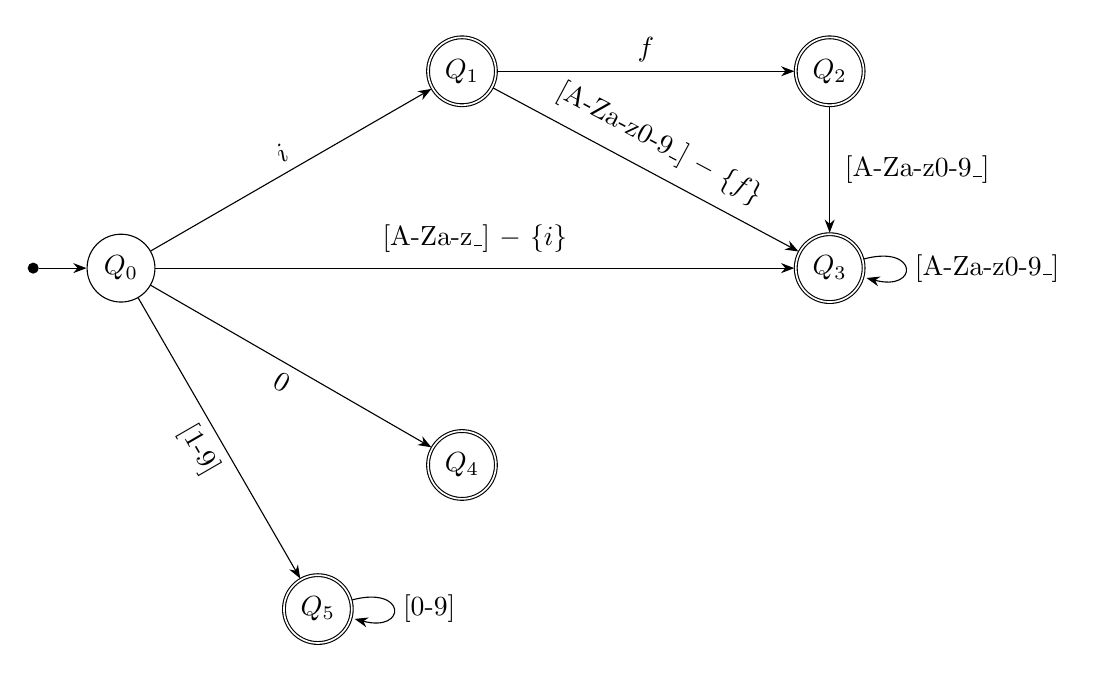
\begin{tikzpicture}[->, >=Stealth, every state/.style={minimum size=8mm}]
\node[state] (Q0) at (0,0) {$Q_0$};
\node[state, accepting] (Q1) at (30:5) {$Q_1$};
\node[state, accepting] (Q2) at (9,2.5) {$Q_2$};
\node[state, accepting] (Q3) at (9,0) {$Q_3$};
\node[state, accepting] (Q4) at (-30:5) {$Q_4$};
\node[state, accepting] (Q5) at (-60:5) {$Q_5$};
\node[circle, fill=black, inner sep=0pt, minimum size=4pt, left=6mm of Q0] (start) {};
\draw (start) -- (Q0);
\path (Q0) edge node[midway, align=center, above, sloped] {$i$} (Q1);
\path (Q0) edge node[midway, align=center, above=2pt] {[A-Za-z\_] $-$ $\{i\}$} (Q3);
\path (Q0) edge node[midway, align=center, below, sloped] {$0$} (Q4);
\path (Q0) edge node[midway, align=center, below, sloped] {[1-9]} (Q5);
\path (Q1) edge node[midway, align=center, above] {$f$} (Q2);
\path (Q1) edge node[midway, align=center, above=2pt, sloped] {[A-Za-z0-9\_] $-$ $\{f\}$} (Q3);
\path (Q2) edge node[midway, align=center, right=2pt] {[A-Za-z0-9\_]} (Q3);
\path (Q3) edge[loop right] node[midway, align=center, right] {[A-Za-z0-9\_]} (Q3);
\path (Q5) edge[loop right] node[midway, align=center, right] {[0-9]} (Q5);
\end{tikzpicture}
\end{center}

\[
Q_0=\varepsilon\mbox{-closure}(\{q_0\})=\{q_0,q_1,q_4,q_6\}.
\]

\begingroup
\renewcommand{\arraystretch}{1.3}
\begin{center}
\begin{tabular}{c|c|l}
DFA State $D$ & Input Character $c$ & DFA Transition $\delta_D(D,c)$ \\
\hline
$Q_0$ & $i$ & $Q_1=\varepsilon\mbox{-closure}(\{q_2,q_5\})=\{q_2,q_5\}$ \\
$Q_1$ & $f$ & $Q_2=\varepsilon\mbox{-closure}(\{q_3,q_5\})=\{q_3,q_5\}$ \\
$Q_0$ & [A-Za-z\_] $-$ $\{i\}$ & $Q_3=\varepsilon\mbox{-closure}(\{q_5\})=\{q_5\}$ \\
$Q_1$ & [A-Za-z0-9\_] $-$ $\{f\}$ & $Q_3=\varepsilon\mbox{-closure}(\{q_5\})=\{q_5\}$ \\
$Q_2,Q_3$ & [A-Za-z0-9\_] & $Q_3=\varepsilon\mbox{-closure}(\{q_5\})=\{q_5\}$ \\
$Q_0$ & $0$ & $Q_4=\varepsilon\mbox{-closure}(\{q_7\})=\{q_7\}$ \\
$Q_0$ & [1-9] & $Q_5=\varepsilon\mbox{-closure}(\{q_8\})=\{q_8\}$ \\
$Q_5$ & [0-9] & $Q_5=\varepsilon\mbox{-closure}(\{q_8\})=\{q_8\}$ \\
\end{tabular}
\end{center}
\endgroup

\end{document}